\subsection{Magnetically forced flow over a backward-facing step}
\label{subsec:backward-facing-step}
To examine the same coupled solver in a channel with a sudden
expansion, we consider
\begin{equation}\label{eq:step-domain}
 \Omega_s=(0,1)\times(0,0.2)\times(0,0.2)
 \setminus\bigl([0,0.2]\times[0,0.2]\times[0,0.1]\bigr).
\end{equation}
The upstream bottom is raised to $z=0.1$ for $x\leq0.2$.
The fluid volume is $0.036$; the inlet $x=0$, $z>0.1$ has area
$0.02$, and the outlet $x=1$ has area $0.04$.
The vertical step face and all remaining boundary faces belong
to the no-slip wall $\Gamma_w$.
The geometry and the dipole locations follow the three-dimensional
step configuration in \cite{DongHuangHuangYang2026}.

The material parameters, zero initial data, zero body sources,
outlet traction, and magnetic and auxiliary boundary conditions are
those stated in \Cref{subsec:straight-channel}, with $\Omega_c$
replaced by $\Omega_s$. The inlet profile is
\begin{equation}\label{eq:step-inlet}
 \bs u_D=\bigl(0.25R(t/0.4)\,16Y(1-Y)Z_s(1-Z_s),0,0\bigr)^{\intercal},
 \qquad Y=\frac{y}{0.2},\quad Z_s=\frac{z-0.1}{0.1}.
\end{equation}
It is supported on the upper half of the inlet and vanishes on
its edges. The inlet and homogeneous wall values are imposed
separately, so the polynomial inlet extension is not applied to the
vertical step face. After ramp-up, the analytic inlet flux is
$1/450$, one half of the straight-channel value because the inlet
area is halved.

The applied field retains \eqref{eq:channel-dipoles}--\eqref{eq:channel-pulse},
with $A=1$, but uses
\begin{equation}\label{eq:step-dipoles}
 \bs x_i^-=(0.2i,-0.2,0.1),\qquad
 \bs x_i^+=(0.2i,0.4,0.1),\qquad i=1,\ldots,4,
 \qquad C_a=7\times10^{-4}.
\end{equation}
The directions remain $\bs d_i^{\pm}=\mp(0,1,0)^{\intercal}$,
with the upper sign corresponding to the upper row.
Thus the waveform, ramp times, period, and phase speed are unchanged,
while the magnetic-source distance and prefactor are explicitly
different. In particular, the relaxation time remains $\tau=0.1$
and the diffusion coefficient remains $\sigma=0.005$.

\paragraph{Mesh and time stepping.}
We use the same second-order spaces, nonlinear midpoint startup,
subsequent extrapolation, quadrature, and solver tolerances as in
the straight channel. The time step is $0.005$ and the simulation
runs to $T=2$.
A conforming tetrahedral mesh is formed from a $5K\times K\times K$
background partition, with the solid cells removed.
Before extracting the fluid mesh, its logical axial coordinate
$\xi$ is mapped to $x$ by the continuous piecewise affine function
specified by
\[
\begin{array}{c|ccccc}
\xi&0&0.1&0.2&0.6&1\\\hline
x&0&0.15&0.2&0.4&1.
\end{array}
\]
This grades the mesh near the step; the transverse coordinates
remain uniform. The resulting mesh has $27K^3$ tetrahedra.
The following visualizations use $K=4$, namely $1728$ tetrahedra.

\paragraph{Field visualization and interpretation.}
\Cref{fig:step-u,fig:step-m,fig:step-omega} use the actual saved
time layer $t=0.715$ (step $143$), rather than a temporally
interpolated state. All three fields use this same time.
The velocity spreads into the larger downstream cross-section after
the step. The magnetization exhibits spatially varying direction
and magnitude, while the angular-velocity distribution is influenced
by the shear near the step and the channel walls.
The displayed angular velocity is the particle spin.

The right panels show the full three-component magnitude on $y=0.1$.
The magnetization arrows are sampled on that same plane; the velocity
and angular-velocity arrows use sparse three-dimensional locations.
Solid-region samples are excluded. The linear arrow scaling and the
color scales are fixed over the stored time interval.
Point values come from the original finite element fields without
RT vertex averaging; interpolation in the filled color surface is
used only for display, not for evaluating finite element norms.
The color limits for $\bs u$, $\bs m$, and $\bs\omega$ are
$0.25$, $0.04$, and $0.04$, respectively.

The $400$-step $K=4$ trajectory passed the stated algebraic and
boundary checks: its maximum recomputed relative residual was
$2.03\times10^{-10}$, and its largest recorded relative inlet--outlet
flux imbalance was $1.12\times10^{-14}$.
A full-interval $K=4$ comparison with $\dt=0.0025$ gave endpoint
relative native volume-$L^2$ differences below $2.9\times10^{-5}$ for
$\bs u$, $\bs m$, $\bs\omega$, and $\bs H$.
These checks assess the implementation and time-step sensitivity.
At the displayed spatial resolution, the figures are a qualitative
illustration; quantitative mesh independence of the step-flow
observables remains to be assessed. In particular, no resolved
reattachment length, corner extremum, or magnetic pumping efficiency
is inferred from these plots. The nonconvex geometry and open
boundary conditions also lie outside the homogeneous convex-domain
setting used in the analysis.

\begin{figure}[!htbp]
\centering
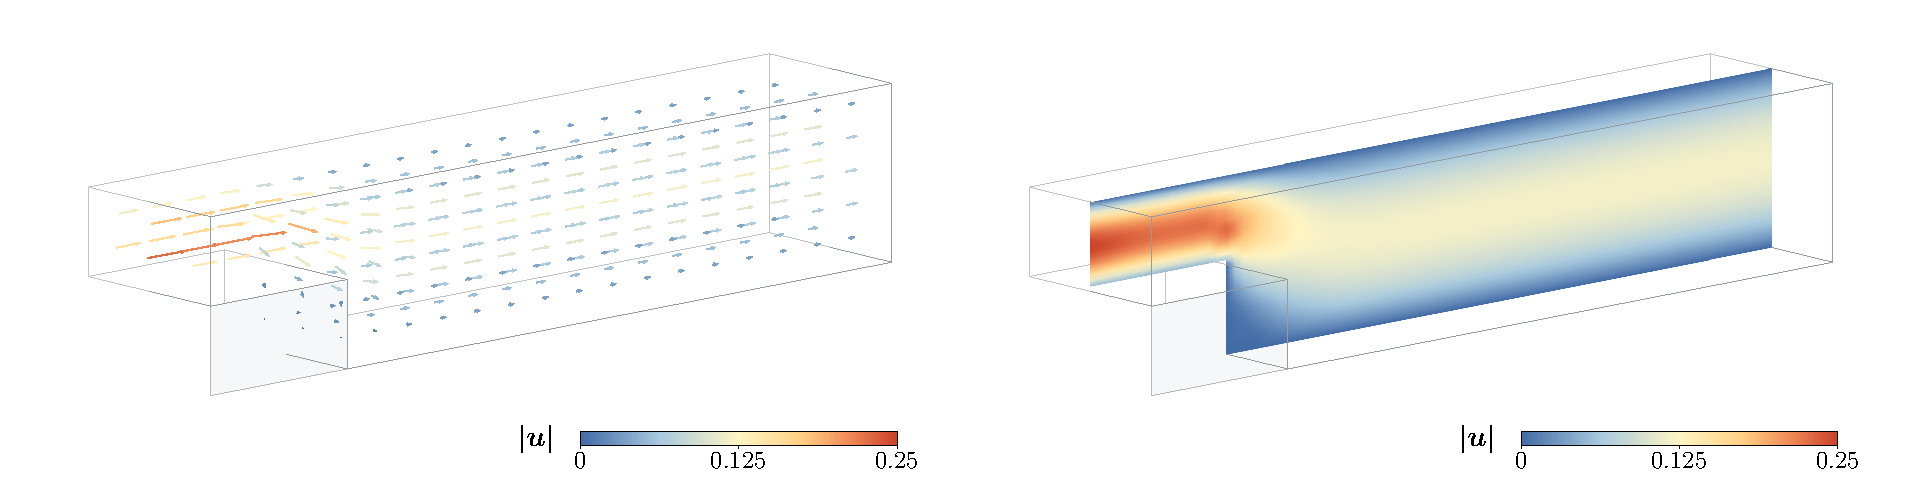
\includegraphics[width=\textwidth]{figures/applications/step_u.pdf}
\caption{Backward-facing-step flow at $t=0.715$ on $K=4$:
velocity vectors (left) and the velocity magnitude on $y=0.1$
(right). The unfilled upstream region is the solid step.}
\label{fig:step-u}
\end{figure}
\begin{figure}[!htbp]
\centering
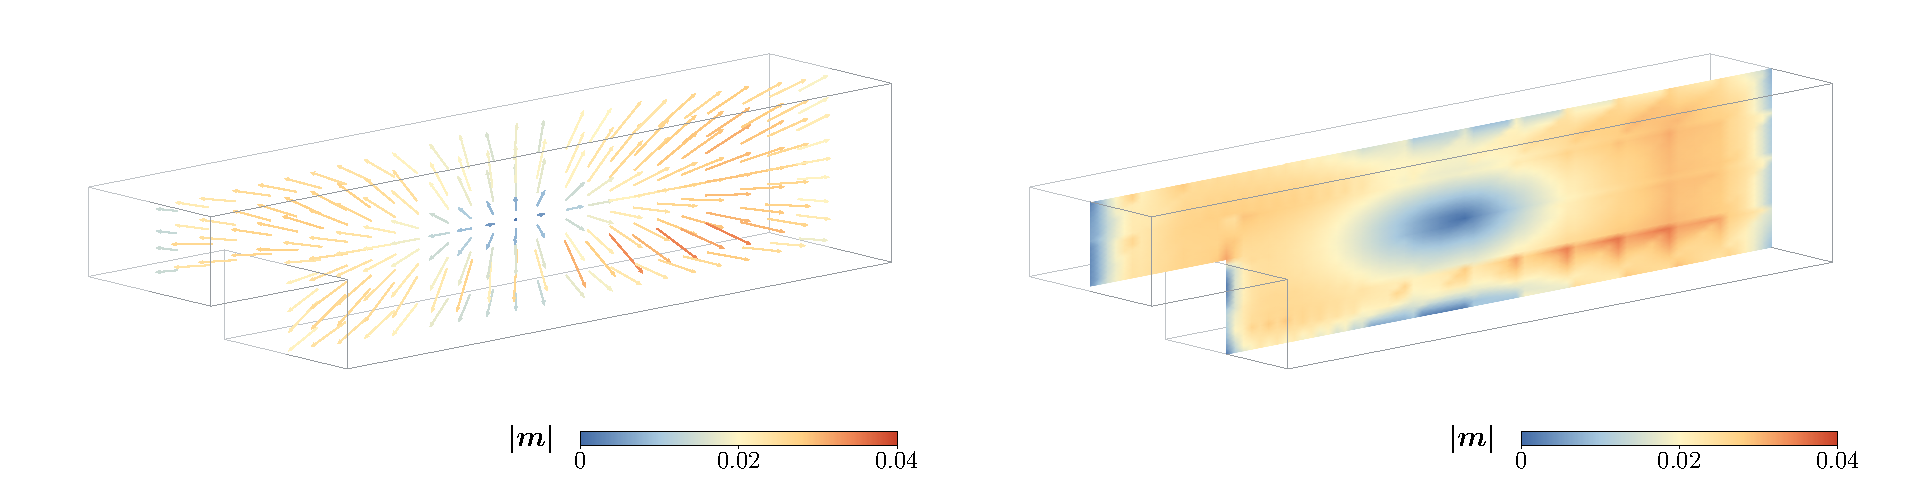
\includegraphics[width=\textwidth]{figures/applications/step_m.pdf}
\caption{Backward-facing-step flow at $t=0.715$ on $K=4$:
magnetization vectors (left) and their full magnitude (right),
both sampled on $y=0.1$.}
\label{fig:step-m}
\end{figure}
\begin{figure}[!htbp]
\centering
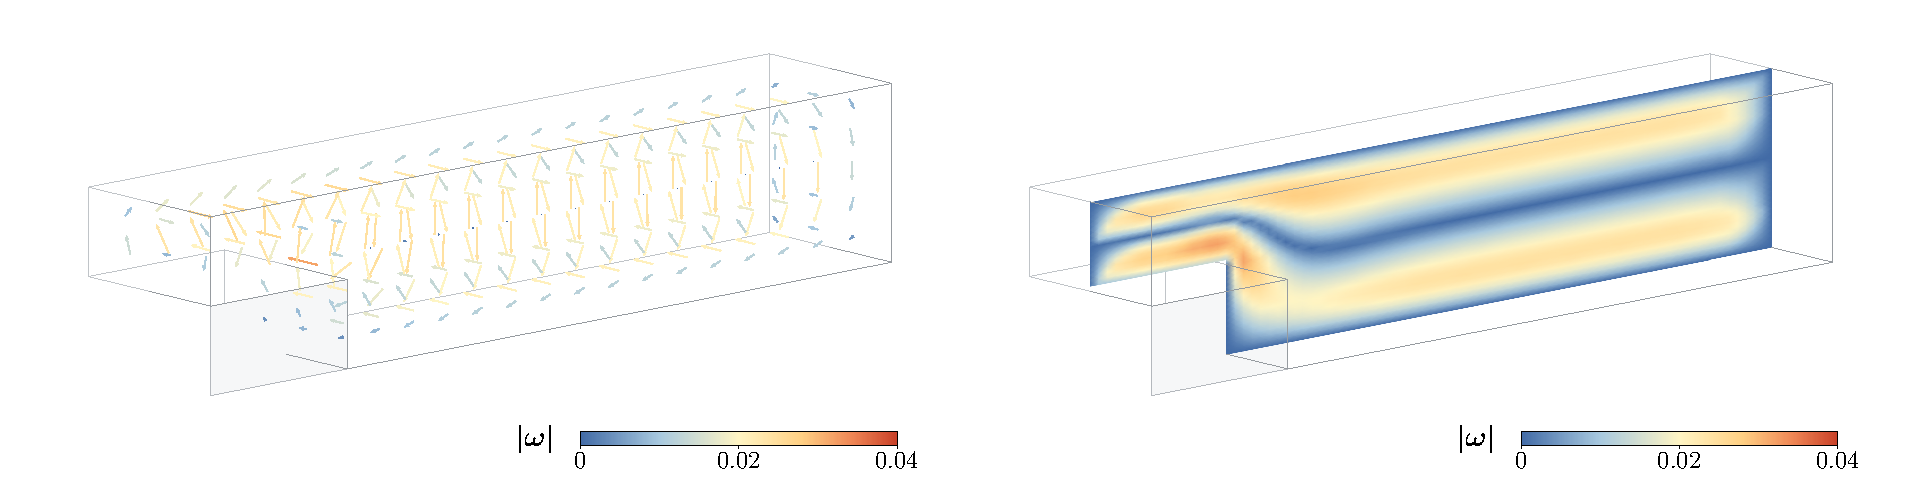
\includegraphics[width=\textwidth]{figures/applications/step_omega.pdf}
\caption{Backward-facing-step flow at $t=0.715$ on $K=4$:
particle angular velocity vectors (left) and their magnitude
on $y=0.1$ (right).}
\label{fig:step-omega}
\end{figure}
\FloatBarrier
